\begin{figure}[h!]
\centering
% \subfloat [Representação de Torta Falsa]{\includegraphics[width=12cm]{./img/representacaoFalsePieGadgetClausula.png}\label{fig:falsePie}}
% \qquad
 \subfloat[$p(e), p(a), p(h)$ adjacent to variables with values $False, True,False$, respectively]{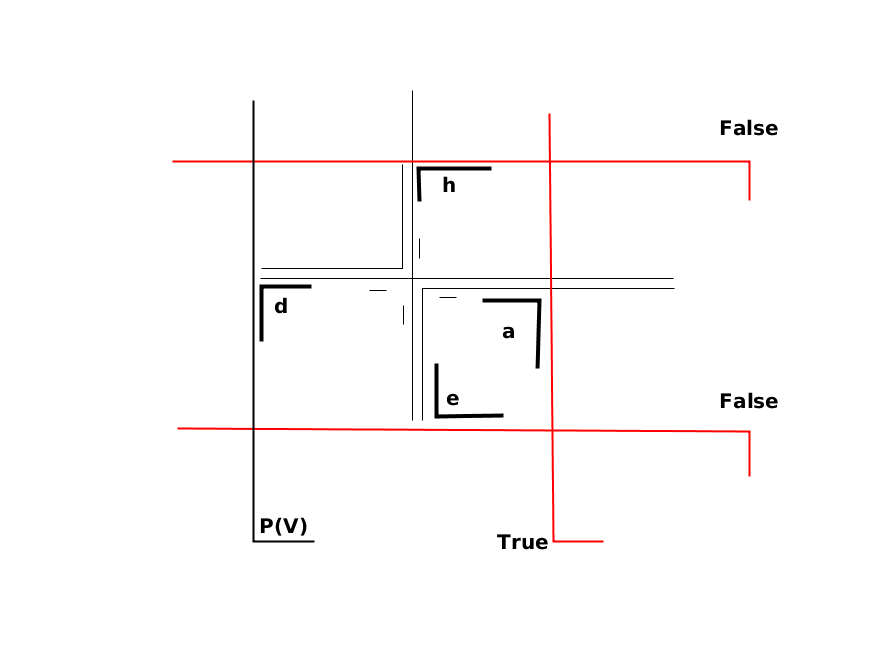
\includegraphics[width=7.8cm]{./img/clausulaGadgetDisposicoesefathf.png}\label{fig:disposicao1}}
 %\qquad
\subfloat[][ $p(e), p(a), p(h)$ adjacent to variables with values $False,False, True$, respectively]{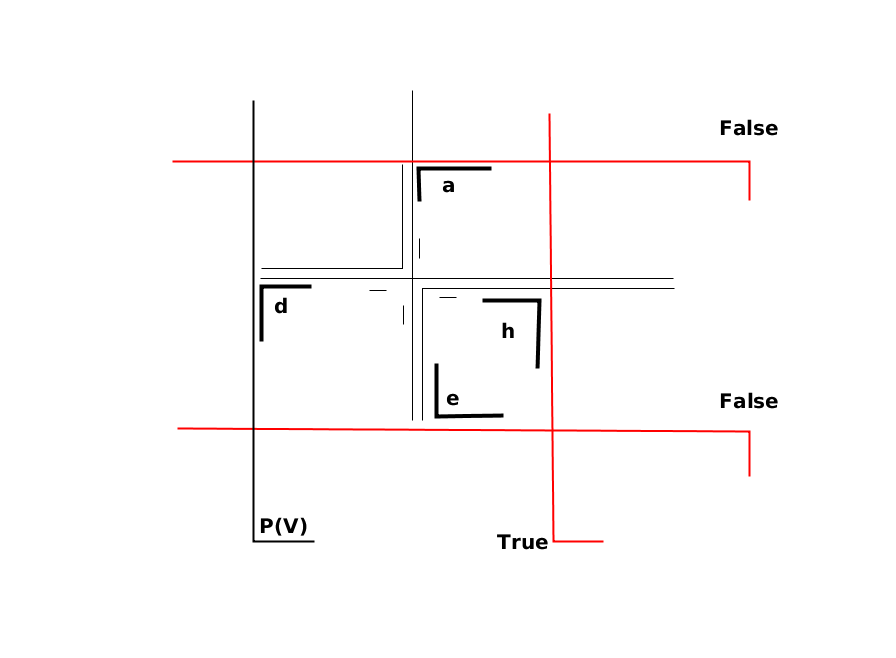
\includegraphics[width=7.8cm]{./img/clausulaGadgetDisposicoesefafht.png}\label{fig:disposicao2}}
\caption{Representation to differents variable arrangements, using structure of false pie.}
\label{fig:disposicoes}
\end{figure}  
  